\clearpage

\section{Game Theory}
\label{sec:background:game_theory}

Game Theory did not exist as a field of own right before von Neumann published the article " On the Theory of Games of Strategy''. This field deals mainly with the study of interactions between rational decision-makers\cite{Neumann1944}. Game Theory knows numerous applications in areas such as Economics, Political Science, Biology, and Artificial Intelligence. 

\subsection{Definition of a Game}
\label{subsec:background:game_theory_definition}

A game ($\Gamma$), is a model of conflict between players characterized by\cite{Osborne2004}\cite{OsbRub94}\cite{Fra2011}:
\begin{itemize}
\item A set of Players: $P=\{1, 2, .., N \}$.
\item For each player there is set of Actions: $X_{i}$
\item There are preferences , for each player, over the set of Actions.
\end{itemize}


The preferences in the previous definitions are defined with resort to the concept of utility, expected utility, or payoff derives from the theory that we can use real numbers (Equation \ref{gt:utilidadesreais}), to model and represent the wants and needs of the players. 

\begin{equation}
u:X\rightarrow\mathbb{R}
\label{gt:utilidadesreais}
\end{equation}

This simplified mathematical model allows to compare different states and rank preferred outcomes. If $u_{i}(x)$ is a utility function for player $i$, and $u_{i}(A)>u_{i}(B)$, that would mean that the player would strictly prefer $A$ over $B$. The concept of expected utility is fundamental to analyse games, as a rational player would try to maximize her expected utility\cite{Neumann1944}\cite{Osborne2004}\cite{Leyton-Brown2008:Essentials_Game_Theory}.


The options a player $i$ has when choosing an action, when the outcome depends not only on their choice (but also on the actions taken by the other players), is referred as strategy $s_{i}$. The set of strategies available to a player is represented by the set $S_{i}$.

When a strategy gives strictly a higher expected utility in comparison to other strategies, we have a strategy that dominates, or a dominant strategy. The mathematical definition of dominance is represented in Equation \eqref{gt:dominant_strategy}; where, for a player $i$, in spite of the strategies chosen by the other players (denoted by $s_{-i}$), there is a strategy $s^{*}$ which gives always an higher expected utility in comparison with other strategies $s^{'}$ available to player $i$.

\begin{equation}
\forall s_{-i}\in S_{-i}[u_{i}(s^{*},s_{-i})>u_{i}(s^{'},s_{-i})]
\label{gt:dominant_strategy}
\end{equation}

The strategy that leads to the most favourable outcome for a player, taking into account other players strategies, is known as best response.

A pure strategy defines deterministically how the player will play the game. In the game represented in Table\ref{tab:2prisionersdillema_tab2} , in a pure strategy, the players either they choose ``Cooperate'' ($C$), or ``Defect'' ($D$). 

If there is a probability distribution associated with probability of playing with a determined pure strategy, we have a mixed strategy. 

There are two standard representations of games:
\begin{itemize}
\item Normal Form - lists what payoffs the players get as a function of their actions as if they all make their moves simultaneously. This games are usually represented by a matrix, for example \ref{tab:2prisionersdillema_tab2}.



\item Extensive Form - extensive form games can be represented by a tree and represent sequential actions.
\end{itemize}

\begin{center}
\begin{table}[h]
\begin{centering}
\begin{tabular}{ccc}
\hline 
 & Player 2: C & Player 2: D\tabularnewline
\hline 
Player 1: C & (2,2) & (0,3)\tabularnewline
Player 1: D & (3,0) & (1,1)\tabularnewline
\hline 
\end{tabular}
\par\end{centering}

\caption{Example of a Normal Form game.}
\label{tab:2prisionersdillema_tab2}
\end{table}
\par\end{center}

A finite game is a game that has a finite set of actions, a finite number or players, and it does not go on indefinitely.

A zero-sum game is a mathematical representation of a system where the gains of the players are completely evened out by the losses of the others; this means that the sum of the utilities of all players will always be zero.





\subsection{Nash Equilibrium}
\label{subsec:background:game_theory_nash_equilibrium}

If we observe the representation of the classic game ``Prisoner's Dilemma'', we can observe that each player has two strategies; either they choose ``Cooperate'' ($C$), or ``Defect'' ($D$). The ``Defect'' strategy, for both players (the game is symmetrical), always yield a higher payoff in spite of the other player's strategy, this means that it is a dominant strategy and also constitutes a best response to the game. If both players chose their best response the final outcome $(D,D)$ becomes an equilibrium solution, more specifically a Nash Equilibrium. 

When all players cannot improve their utility by changing their strategy unilaterally, we have an equilibrium point. This equilibrium point is named after John Nash, who proved that it exists at least one mixed strategy Nash equilibrium in a finite game\cite{nash50}\cite{Nash51}. This concept is used to analyse game where several decision makers interact simultaneously and the final outcome depends on the players strategy\cite{Osborne2004}.

In order to compute a mixed strategy Nash Equilibrium in a 2-player 2 actions game, we need to define the probability distribution $P(C)=q$, $P(D)=1-q$ that makes player 1 indifferent to the whether player 2 decides to Cooperate or to Defect, and the probability distribution $P(C)=p$, $P(D)=1-p$ that makes player 2 indifferent to whether player 1 decides to Cooperate or to Defect. In the game represented in Table \ref{tab:2pennyflip_tab2} the  mixed strategies $(\frac{1}{3} , \frac{2}{3})$ and $(\frac{2}{3} , \frac{1}{3})$ are Nash Equilibria.

\begin{center}
\begin{table}[h]
\begin{centering}
\begin{tabular}{ccc}
\hline 
 & Player 2: C & Player 2: D\tabularnewline
\hline 
Player 1: C & (2,1) & (0,0)\tabularnewline
Player 1: D & (0,0) & (1,2)\tabularnewline
\hline 
\end{tabular}
\par\end{centering}

\caption{Example of a Normal Form game. The mixed strategies $(\frac{1}{3} , \frac{2}{3})$ and $(\frac{2}{3} , \frac{1}{3})$ are Nash Equilibria for this game. }
\label{tab:2pennyflip_tab2}
\end{table}
\par\end{center}

When there is at least a Nash Equilibrium when the players choose pure strategies we have a a strictly determined game\cite{Leyton-Brown2008:Essentials_Game_Theory}

In an extensive form game we have a concept of sub-game perfect Nash equilibrium, when a strategy is a Nash equilibrium for all sub-games in the original game\cite{Leyton-Brown2008:Essentials_Game_Theory}.

\subsection{Prisoner's Dilemma}
\label{sebsec:related_work_prisioners_dillama}

The Prisoner's Dilemma is a classic example of a game that can be represented
in normal form\cite{Osborne2004}. This problem has received a great deal of attention
because, in its simple form, rational individuals will seem to deviate
from solutions that would represent the best social interest,
the Pareto Optinal solution. In this game the Pareto Optimal solution
is not a Nash Equilibrium. The Prisoner's Dilemma can be formulated
as it follows:

\begin{quotation}

Two suspects of being partners in a crime are arrested. The police
needs more evidence in order to prosecute the prisoners. So each
prisoner is locked in solitary confinement and has no means of communicating
with the other suspect. The police will then try to extort a confession
from the prisoners. A bargain will be proposed to the suspects:
\begin{itemize}
\item If the suspect testifies against the other suspect (Defects) and the other denies, he will
go free and the second will get three years sentence.
\item If they both testify against one another (both Defect), both will
be convicted and they will get two years.
\item In case both suspects deny the involvement (both Cooperate) of the
other, they will get a one year sentence.
\end{itemize}
\end{quotation}

A matrix representation of the problem is in Table \ref{tab:prisionersdillema_tab1}, here the payoff represented by the letter $R$ would be the standard reward for the game, $T$ would be the temptation to deviate from a cooperation profile, $P$ represents the punishment when both entities do not cooperate, and finally $S$ would be a sucker's payoff. A particular case for this problem is represented in Table \ref{tab:prisionersdillema_tab2}. In each cell of the matrix we have a pair of the expected utility for the players for every outcome. A higher utility represents a more desirable state.

In this game the Pareto Optimal solution happens when both players chose to Cooperate (the pair (2,2) in Table \ref{tab:prisionersdillema_tab2}). However both players have the incentive to Defect, because regardless what the opponent chooses they will have always a strictly higher payoff. Defecting becomes a dominant strategy in the Prisioner's Dillema and the outcome $(Defect, Defect)$ is a Nash Equilibrium to the game. 

\begin{center}
\begin{table}[h]
\begin{centering}
\begin{tabular}{ccc}
\hline 
 & Player 2: C & Player 2: D\tabularnewline
\hline 
Player 1: C & (R,R) & (S,T)\tabularnewline
Player 1: D & (T,S) & (P,P)\tabularnewline
\hline 
\end{tabular}
\par\end{centering}

\caption{The canonical normal form representation for the Prisoner's Dilemma must respect $T>R>P>S$.}
\label{tab:prisionersdillema_tab1}
\end{table}
\par\end{center}

\begin{center}
\begin{table}[h]
\begin{centering}
\begin{tabular}{ccc}
\hline 
 & Player 2: C & Player 2: D\tabularnewline
\hline 
Player 1: C & (2,2) & (0,3)\tabularnewline
Player 1: D & (3,0) & (1,1)\tabularnewline
\hline 
\end{tabular}
\par\end{centering}

\caption{One possible normal form representation of Prisoner's Dilemma.}
\label{tab:prisionersdillema_tab2}
\end{table}
\par
\end{center}



\subsection{Pareto Optimal}
\label{subsec:background:game_theory_pareto_optimal}

From the point of view of an observer outside the game system some outcomes may seem better than others. For example on the game represented in Table \ref{tab:2prisionersdillema_tab2} (Prisioners' Dilemma), the outcome $(C,C)$ seems better than the outcome $(D,D)$ because it provides a strictly higher utility to the players. However we know that the outcome $(D,D)$ is the Nash Equilibrium of the game. If both players use their best response their outcome might not be the best outcome for both players.

When it is impossible to improve the payoff of a player without lowering another player's expected utility we have a Pareto Optimal solution.

For example if we have two players and $10$ units of a finite resource to distribute among the players, a Pareto optimal solution is $(5,5)$. Any other attempt to redistribute where the sum of the resource isn't $10$ -$(1,4)$, $(2,3)$, etc...- could still be improved.


\clearpage
\section{Quantum Game Theory}
\label{sec:background_quantum_game_theory}



In the article ``Quantum information approach to normal representation of extensive games''\cite{Fra2011a}, the authors propose a representation
for both normal and finite extensive form games\cite{Fra2011}. This definition is based on the premise that any strategic game can be represented as an extensive form game where all the players have no knowledge about the actions taken by other players. 

The representation assumes that for each action that a player can make in the game there are only two possible measurable outcomes. For example while voting on a referendum in which the question is "Should the state declare war on country X?" despite the method using for voting the final answer is revealed as a ""yes"" or ""no"".
In Quantum Game Theory we model an action as a qubit which is manipulated by the player. 


A game in this
form is represented by a six-tuple\eqref{eq:quantum_game_six_tuple},
where:

\begin{equation}
\Gamma=(\mathcal{H}^{2^{a}},\: N,\:\vert\psi_{in}\rangle,\:\xi,\:\{\mathcal{U}_{j}\},\:\{E_{i}\})\label{eq:quantum_game_six_tuple}
\end{equation}

\begin{itemize}
\item $a$ is the number of actions (qubits), in the game; 
\item $\mathcal{H}^{2^{a}}$ is a $2^{a}$-dimensional Hilbert space constructed
as $\otimes_{j=1}^{a}\mathbb{C}^{2}$, with basis $\mathcal{B}$;
\item $N$ is the number of players;
\item $\vert\psi_{in}\rangle$ is the initial state of the compound-system
composed by $a$ qubits: $\vert\varphi_{1}\rangle,\:\vert\varphi_{2}\rangle, ..., \vert\varphi_{j}\rangle, ..., \vert\varphi_{a}\rangle$;
\item $\xi$ is a mapping function that assigns each action to its respective player;
\item For each qubit $j$, $\mathcal{U}_{j}$ is a subset of unitary operators from $\mathsf{SU}(2)$ (the general for the 2 dimensional Special Unitary Group is presented in Equation \eqref{eq:general_unitary_special_one}).
These operators can be used by the player to manipulate her qubit(s);
\begin{equation}
\begin{split}
\mathcal{U}_{j}(w,x,y,z)=w.I + ix.\sigma_{x} + iy.\sigma_{y} + iz.\sigma_{z}, \\  w,x,y,z \in \mathbb{R} \wedge  
w^2 + x^2 + y^2 + z^2 =1 
\end{split}
\label{eq:general_unitary_special_one}
\end{equation}
\item Finally, for each player $i$, $E_{i}$ is a utility functional that
specifies her payoff. This is done by attributing a real number (representing a expected utility $ u_{i}(b)$, in \eqref{eq:quantum_game_definition_payoff_func}), to the measurement for the projection of the final state (\eqref{eq:quantum_game_definition_move}), on a basis from the $\mathcal{B}$\eqref{eq:quantum_game_definition_payoff_func}.\end{itemize}



\begin{equation}
E_{i}=\sum_{b \in \mathcal{B}} u_{i}(b)\vert \langle b\vert \psi_{fin}\rangle\vert^{2}, u_{i}(b) \in \mathbb{R}
\label{eq:quantum_game_definition_payoff_func}
\end{equation}

The strategy of a player $i$ is a map $\tau_{i}$ which assigns a
unitary operator $U_{j}$ to every qubit $j$ that is manipulated
by the player (\inputencoding{latin1}{$j$$\in\xi^{-1}(i)$}\inputencoding{latin9}).
The simultaneous move is represented in \eqref{eq:quantum_game_definition_move}.

\begin{equation}
\vert\psi_{fin}\rangle=\otimes_{i=1}^{N}\otimes_{j\in\xi^{-1}(i)}\mathcal{U}_{j}\vert\psi_{in}\rangle
\label{eq:quantum_game_definition_move}
\end{equation}

The tensor product of all the operators chosen by the players is referred as a super-operator, which act upon the game system.

\begin{comment}
In the article "Quantum Games and Quantum Strategies"\cite{Eisert2008}, the authors describe a quantization scheme for the Prisoner's Dilemma game. The way the initial state, $\vert\psi_{in}\rangle$, is set-up in the game system provide a way to entangle the game system, thus allowing the study of this phenomenon. For a $2$-player game, this is accomplished using Equation \eqref{eq:2_4:estado_inicial_prisioneiro}. $\mathcal{J}$ is a matrix exponential that is chosen because it can commute with a super-operator, made from the subset of unitary operators that contains the identity matrix and the Bit-flip Pauli matrix\cite{citeulike:10961388}. According to \cite{Eisert2008}, the parameter $\gamma$ becomes a way to measure the entanglement in the system.

\begin{equation}
\label{eq:2_4:matrix_exponencial_esoterica}
\mathcal{J}=exp\left\{ i\frac{\gamma}{2}\left[\begin{array}{cc}
0 & 1\\
1 & 0
\end{array}\right]\otimes\left[\begin{array}{cc}
0 & 1\\
1 & 0
\end{array}\right]\right\}
\end{equation} 

\begin{equation}
\label{eq:2_4:estado_inicial_prisioneiro}
\begin{split}
\vert\psi_{in}(\gamma)\rangle=exp\left\{ i\frac{\gamma}{2}\left[\begin{array}{cc}
0 & 1\\
1 & 0
\end{array}\right]\otimes\left[\begin{array}{cc}
0 & 1\\
1 & 0
\end{array}\right]\right\} \vert00\rangle \\
=cos(\frac{\gamma}{2})\vert00\rangle+isin(\frac{\gamma}{2})\vert11\rangle,\gamma\in(0,\pi)
\end{split}
\end{equation}

\end{comment}


\subsection{Quantum Prisoner's Dilemma}
\label{subsubsec:quantum_prisioners_dillema}

The importance of the Prisoner's Dilemma for the study of Game Theory made it a prime target for investigation in Quantum Game Theory. The problem has been modelled several times \cite{Eisert2008}\cite{Letters2002}. Therefore we will use it in order to exemplify and consolidate the definition described above, in Section \ref{sec:background_quantum_game_theory}\cite{Fra2011a}. 

Each player $i$ in the quantum version of Prisoner's Dilemma will be able to manipulate one qubit ($\varphi_{1}$ and $\varphi_{2}$) in Equations \eqref{eq:quantum_prisioner_m1} and \eqref{eq:quantum_prisioner_m2}, with the unitary operators (shown in Equation \eqref{eq:operators_prisioneiros_quanticos}). The  classical strategies: Cooperate (C), and Defect (D). $C$ is represented in the sub-set $\mathcal{U}_{j}$ (Equation \eqref{eq:operators_prisioneiros_quanticosmiaurons}) . $D$, also known as the Bit-flip operator ($\sigma_{x}$), is not represented in the restricted space proposed in \cite{Eisert2008}\cite{Fra2011a}. $D^{y}$ is an alternative to $D$ in the sub-set $\mathcal{U}$.

\begin{equation}
\varphi_{1}=a_{0}\vert0\rangle+a_{1}\vert1\rangle,\sum_{i=0}^{1}\vert a_{i}\vert^{2}=1
\label{eq:quantum_prisioner_m1}
\end{equation}


\begin{equation}
\varphi_{2}=b_{0}\vert0\rangle+b_{1}\vert1\rangle,\sum_{j=0}^{1}\vert b_{j}\vert^{2}=1
\label{eq:quantum_prisioner_m2}
\end{equation}

\begin{equation}
\mathcal{U}_{j} ( \theta,\phi) = \left[\begin{array}{cc}
cos(\frac{\phi}{2}) & e^{i\phi}sin(\frac{\phi}{2})\\
-e^{-i\phi}sin(\frac{\phi}{2}) & cos(\frac{\phi}{2})
\end{array}\right] , j \in \{ 1, 2\}, \theta \in ( 0, \pi ) , \phi \in ( 0, \frac{\pi}{2})
\label{eq:operators_prisioneiros_quanticos}
\end{equation}

\begin{equation}
\begin{cases}C= 
U_{j}(0, 0)=\left[\begin{array}{cc}
1 & 0\\
0 & 1
\end{array}\right]\\
D=\left[\begin{array}{cc}
0 & 1\\
1 & 0
\end{array}\right] \\
D^{y}= U_{j}(\pi, 0)=\left[\begin{array}{cc}
0 & 1\\
-1 & 0
\end{array}\right]
\end{cases} , j \in \{ 1, 2 \}
\label{eq:operators_prisioneiros_quanticosmiaurons}
\end{equation}

The system that holds the game is represented in a $\mathcal{H}^{4}$. Each basis ($\vert 1\rangle, \vert 2\rangle, \vert 3\rangle, \vert 4\rangle$), represents a final outcome as Table \ref{tab:prisioners_m} suggests.

\begin{table}
\begin{centering}
\begin{tabular}{ccc}
\hline 
$\bigotimes$ & C-$\vert 0\rangle$ & D-$\vert 1\rangle$\tabularnewline
\hline 
C-$\vert 0\rangle$ & $\vert 0,0\rangle$ & $\vert 0,1\rangle$\tabularnewline
D-$\vert 1\rangle$ & $\vert 1,0\rangle$ & $\vert 1,1\rangle$\tabularnewline
\hline 
\end{tabular}
\par\end{centering}

\caption{Construction of the basis for the game space; $\mathcal{H}^{4}$.}
\label{tab:prisioners_m}
\end{table}



The fundamental difference from the classical version lies in the way the initial state is formulated in Equation and the strategies the players might use\eqref{eq:estado_inicial_prisioneiro}. We will entangle our state by applying the gate $\mathcal{J}$ \cite{Letters2002}\cite{Eisert2008}. 

The parameter $\gamma$ becomes a way to measure the entanglement in the system\cite{Eisert2008}.

\begin{equation}
\label{eq:matrix_exponencial_esoterica}
\mathcal{J}=exp\left\{ i\frac{\gamma}{2}\left[\begin{array}{cc}
0 & 1\\
1 & 0
\end{array}\right]\otimes\left[\begin{array}{cc}
0 & 1\\
1 & 0
\end{array}\right]\right\}
\end{equation} 

\begin{equation}
\label{eq:estado_inicial_prisioneiro}
%\vert \psi_{in}(\gamma) \rangle= cos( \frac{\gamma}{2})\vert 00\rangle+ isin(\frac{\gamma}{2})\vert 11 \rangle, \gamma \in (0,\pi)
\begin{split}
\vert\psi_{in}(\gamma)\rangle=exp\left\{ i\frac{\gamma}{2}\left[\begin{array}{cc}
0 & 1\\
1 & 0
\end{array}\right]\otimes\left[\begin{array}{cc}
0 & 1\\
1 & 0
\end{array}\right]\right\} \vert00\rangle \\
=cos(\frac{\gamma}{2})\vert00\rangle+isin(\frac{\gamma}{2})\vert11\rangle,\gamma\in(0,\pi)
\end{split}
\end{equation}

\begin{equation}
\vert\psi_{fin}\rangle= \mathcal{J}^{\dagger} \otimes_{i=1}^{2}\mathcal{U}_{i}\vert\psi_{in}\rangle
\label{eq:finalstate_prisioneersdilemma}
\end{equation}

The entanglement in quantum game theory can be viewed as an intrinsic unbreakable contract. Furthermore measuring an entangled state will cause the wave function that describes the state to collapse. Before measuring the final result we will de-entangle the system by applying the operator $\mathcal{J}^{\dagger}$, as shown in Equation \eqref{eq:finalstate_prisioneersdilemma}.

The utility functions for each player is calculated by projecting the final state in each base and attributing a real number to each measurement, as in equation.
In order to compare a classical version with this quantum model, the real numbers assigned are those in the classical example in Table \ref{tab:prisionersdillema_tab1}, and the basis are presented in Table \ref{tab:prisioners_m}.

\begin{equation}
E_{0}(\vert\psi_{fin}\rangle)=2\times\vert\langle00\vert\psi_{fin}\rangle\vert^{2}+3\times\vert\langle10\vert\psi_{fin}\rangle\vert^{2}+1\times\vert\langle11\vert\psi_{fin}\rangle\vert^{2}
\end{equation}


\begin{equation}
E_{1}(\vert\psi_{fin}\rangle)=2\times\vert\langle00\vert\psi_{fin}\rangle\vert^{2}+3\times\vert\langle01\vert\psi_{fin}\rangle\vert^{2}+1\times\vert\langle11\vert\psi_{fin}\rangle\vert^{2}
\end{equation}



The gate $\mathcal{J}$ is chosen to be commutative with the super-operators created by the tensor product of the classical strategies C and D: $ [ \mathcal{J} , C \otimes C ] = 0 $, $ [ \mathcal{J} , C \otimes D ] = 0 $, $ [ \mathcal{J} , D \otimes C ] = 0 $, and $ [ \mathcal{J} , D \otimes D ] = 0 $. 

This condition implies that any pair of strategies in the sub-set $S_{0} = \{ \mathcal{U} ( \theta , 0) , \theta \in (0, \pi) \}$ is the equivalent of a classical mixed strategy when $\gamma = 0$; the joint probability associated with measuring a outcome $(\delta_{1}, \delta_{2}) \in \{ (C, C), (C, D), (D, C), (D, D) \} $ ( $ P( \delta_{1} , \delta_{2} ) = { \vert \langle \delta_{1} , \delta_{2} \vert \psi_{fin} \rangle \vert }^{2} $ ), becomes $ P( \delta_{1} , \delta_{2} ) =P( \delta_{1} ) P( \delta_{2})$, with $P(C) = cos^{2}(\frac{ \theta }{2})$, and $P(D) = 1 - P(C)$\cite{Eisert2008}.

If the parameter $\phi$ in the operator $U_{j}(\theta ,\phi)$ and the entanglement coefficient differ from $0$ we are able to explore quantum strategies that have no counterpart in the classical domain.

\cite{Eisert2008} finds that the pair of strategies $( \mathcal{U}( 0 , \frac{\pi}{2}), \mathcal{U}( 0 , \frac{\pi}{2}))$ for $\gamma = \frac{\pi}{2}$ yield  a payoff of $(2,2)$, which is a Nash equilibrium and it is Pareto Optimal when we have a restricted space described by $\mathcal{U}$\eqref{eq:operators_prisioneiros_quanticos}. If we allow the operator $D$\eqref{eq:operators_prisioneiros_quanticosmiaurons}, however, according to \cite{Letters2002} there is no quantum pure strategy Nash Equilibrium, when the entanglement is maximal, $\mathcal{U}(\pi, 0)$ is the optimal counter-strategy for $C$ (represented by the identity matrix), $\mathcal{U}(0, \frac{\pi}{2})$ is the optimal counter strategy for $\mathcal{U}(\pi, 0)$, $D$ becomes the optimal counter-strategy for $\mathcal{U}(0, \frac{\pi}{2})$, and $C$ becomes an optimal counter strategy for $D$\cite{Du}.




\begin{comment}

\begin{table}[ht!]
\begin{center}
\begin{tabular}{cc}
  \num\putindeepbox[7pt]{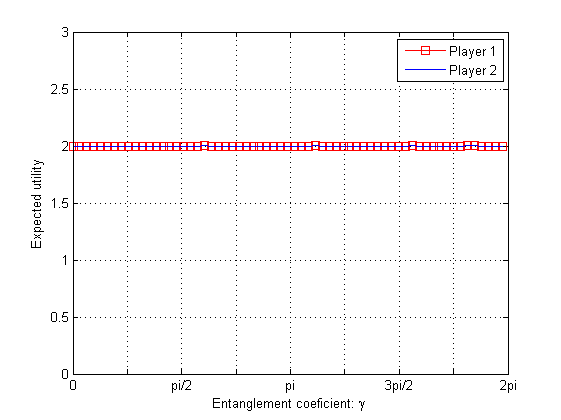
\includegraphics[scale=0.46]{prisionersdillema/II.PNG}}
    & \num\putindeepbox[7pt]{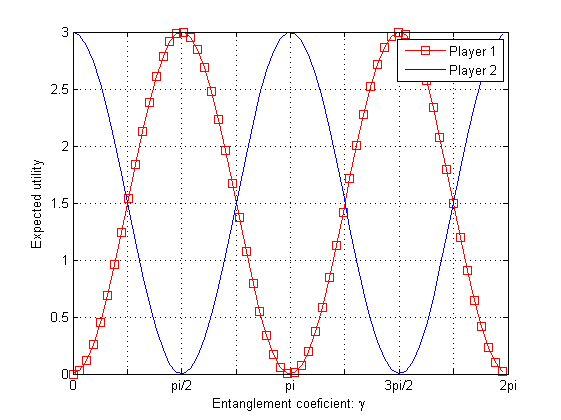
\includegraphics[scale=0.46]{prisionersdillema/InotI.PNG}} \\
  \num\putindeepbox[7pt]{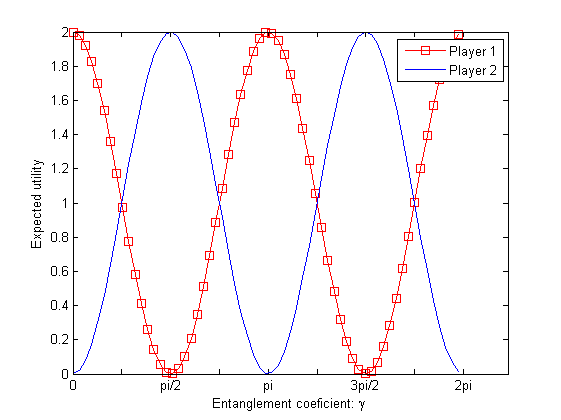
\includegraphics[scale=0.46]{prisionersdillema/notII.PNG}}
    & \num\putindeepbox[7pt]{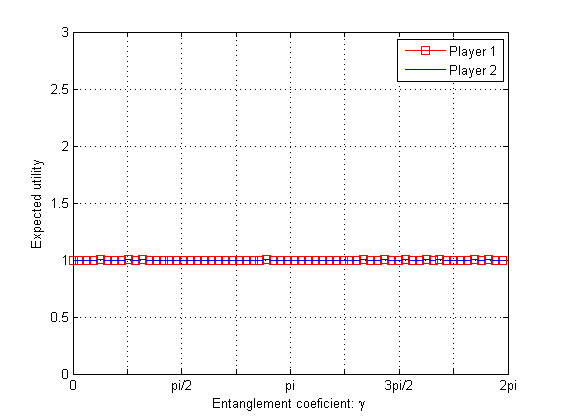
\includegraphics[scale=0.46]{prisionersdillema/notInotI.PNG}} \\
\end{tabular}
\caption{Expected utility for players 1 and 2 giving the entanglement coefficient $\gamma$ used in preparing the initial state. a) Player 1: Cooperates, Player 2: Cooperates;
b) Player 1: Cooperates, Player 2: Defects; c) Player 1: Defects, Player 2: Cooperates; d) Player 1: Defects, Player 2: Defects. }
\label{tab:prisiones_m_4}
\end{center}
 \end{table}

\end{comment}





